\chapter{Design and Methodology}
\label{cha:methodology}
In this chapter we present the tools and techniques used in our experimental analysis and detail their application. We partition our approach into three categories, each focused on addressing a particular section of our overarching hypothesis. Firstly in \cref{sec:Msimenvironment} we detail the network simulation environment, data sets, and produced tools. In this section we also give a high-level implementation overview of the network, probe paths, and other data structures.\par
Secondly in \cref{sec:Mnetworkprobing} we cover our approach to testing sub-hypothesis one, that network tomography enables inference of node level packet delay metrics within stochastically routing networks. Specifics are also given of how network tomography has been applied and subsequently evaluated with respect to its ability as a tool for inferring node level metrics.\par
Thirdly in \cref{sec:MPDMinferencevalid} we conduct an experiment on a synthetic network to validate our use of network tomography to infer router level packet delay metrics. We assess the impact of variable number of probe packets on the accuracy of network tomography. This was done to inform design decision surrounding the frequency with which monitors should generate probe packets.\par
Fourthly in \cref{sec:MNefidentification} we give an overview of our approach to determining router level nefarious hold probability. We conduct experiments on synthetic network topologies to determine the impact of probabilistic packet delaying by routers on obtainable metrics. We identify two candidate metrics of average packet delay (PDA), and packet delay variance (PDV). We then compare these to determine the most appropriate metric to use in our classification.\par
We then present our experimental methodology around assumptions underpinning the development of our three classifiers. Additionally, we present techniques used to evaluate the efficacy of each classifier and enumerate three real-world use cases to quantitatively compared classifier performance.\par
Finally in \cref{sec:Moptprobing} we segment the complex process of network tomography using a novel representation that we refer to as the \textit{tomographic pipeline}. We then cover our implementation of two optimisations to this tomographic pipeline.

\section{Simulation Environment and Tools}
\label{sec:Msimenvironment}
This section details network topology data sets, network traffic data generation, tools for analysis, and developed software packages for evaluation of our overarching hypothesis.In \cref{ssec:Mdatasets} we detail the data used for real-world ISP network analysis. In \cref{ssec:Mdataprocessing} alterations and additions to the data sets are addressed, along with methods of traffic generation and probing data. Functionality of the produced software is listed in \cref{ssec:Msoftware}. Implementation details for all classes and analysis scripts can be found in \cite{sylvester_millar_real_2021}.

\subsection{Data Sets}
\label{ssec:Mdatasets}
Real-world topology data sets are from the SNDLib project (\cite{orlowski_sndlib_2007}) and the Internet Topology Zoo project (\cite{knight_internet_2011}). We have selected three national ISP topologies for analysis. Details and plots of these networks are shown in \cref{tbl:Mrealnetworkattributes} and \cref{fig:MISPplots} respectively. These topologies were selected as they have a high connectivity (without being fully connected) and large number of nodes (>15) compared to other topologies within the data set. We believe this combination represents real-world scenarios where network tomography can provide useful results with, non-trivial performance improvements over conventional monitoring methods (such as SNMP).\par
A synthetic seven-router network was also used for initial data exploration. A worked example of network tomography using this network, and a diagram of the topology, are provided in \cref{sec:Mnetworkprobing}.\par
\begin{table}
    \centering
    \begin{tabular}{@{}cccccccc@{}} 
      \toprule
      &&&&&\multicolumn{3}{c}{Router Degree}\\
      \cmidrule{6-8}
      Name & Region & Year & \# Routers & \# Links & Min & Max & Mean \\
      \midrule
      Nobel & Germany & 2005 & 17 & 26 & 2 & 6 & 3.05\\
      Free & France & 2005 & 25 & 45 & 2 & 10 & 3.6\\
      CPLEX & Norway & 2005 & 27 & 51 & 2 & 6 & 3.78\\
      \bottomrule
    \end{tabular}
    \caption{Real world network ISP topology attributes.}
    \label{tbl:Mrealnetworkattributes}
  \end{table}

\noindent
\begin{figure}
    \centering
    \begin{subfigure}{0.475\textwidth}
        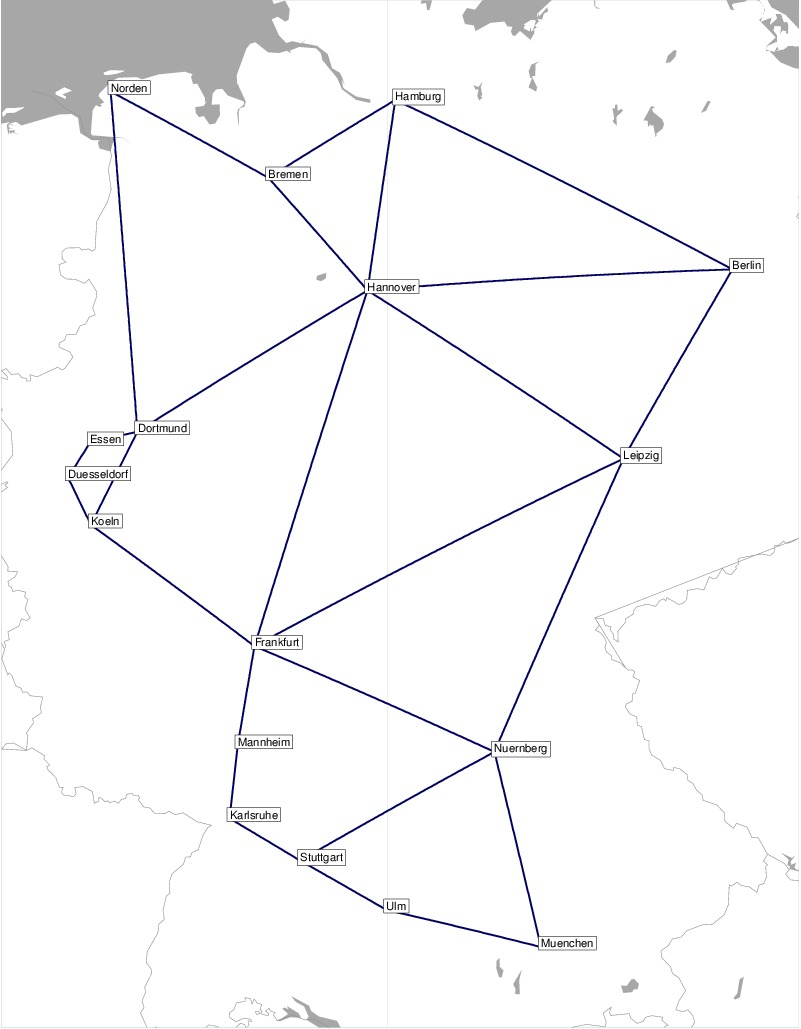
\includegraphics[width=\textwidth]{figs/methodology/nobel-germany.jpg}
        \caption{Nobel Topology.}
    \end{subfigure}
    
    \begin{subfigure}{0.475\textwidth}
        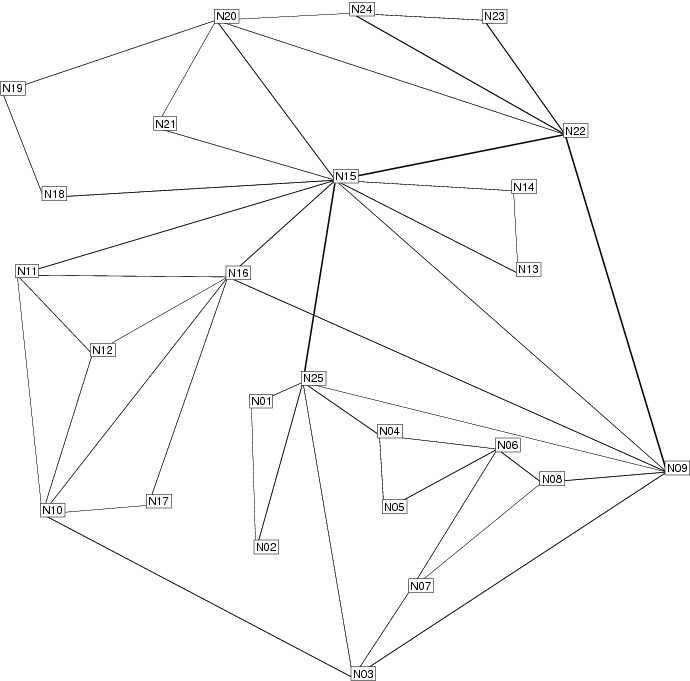
\includegraphics[width=\textwidth]{figs/methodology/france.jpg}
        \caption{Free Topology.}
    \end{subfigure}
    \begin{subfigure}{0.475\textwidth}
        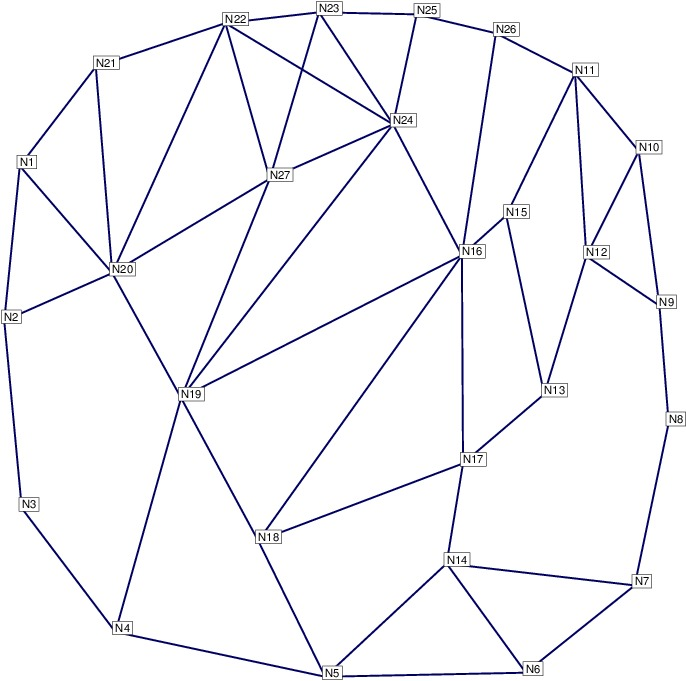
\includegraphics[width=\textwidth]{figs/methodology/norway.jpg}
        \caption{CPLEX Topology.}
    \end{subfigure}
    \caption[Plots of each real-world ISP topology.]{Plots of each real-world ISP topology (from \cite{knight_internet_2011} and \cite{orlowski_sndlib_2007}).}
    \label{fig:MISPplots}
\end{figure}

\subsection{Data Processing}
\label{ssec:Mdataprocessing}
Data from both the SNDlib and Internet Topology Zoo projects are stored in a range of bespoke XML and GraphML formats. To maximise speed of the network simulation, these formats were parsed into a graph object in the Python iGraph library (\cite{csardi_igraph_2006}). Nodes and links from the topology data sets are represented as iGraph vertices and links respectively. All Python objects were stored using Python's pickle module (\cite{van_rossum_python_2020}).\par
An object representing each network device (\textit{i.e. router or switch}) is stored as an attribute of each iGraph vertex along with an ID to account for iGraph's dynamic object indexing. Each network device stores an array of packets received each timestep, shuffling and appending elements from this array to its queue buffer to emulate temporal ambiguity in receiving packets. As each packet is an instance of a UDP packet class, additional packets are silently dropped once the buffer queue reaches capacity.\par
Despite best efforts, network traffic data could not be acquired for systems with robustly mapped topologies and probabilistically delaying routers. Due to this, traffic was generated at simulation run-time from switches attached to routers. Each switch has a fixed probability of sending a packet (with a random destination) to its attached router every timestep. As the number of packets received by routers follows a Poisson distribution (see \cref{sssec:Itrafficsimulation}), the number of switches attached to each router is selected at random from the Poisson class of NumPy's random library.\par
UDP traffic is stochastically routed through the network using a link state (\textit{LS}) protocol. Link state advertisements are broadcast at the start of the simulation. To allow for the routing tables to stabilise, the network is not probed for the first 5\% of the simulation. LS advertisements are sent periodically throughout the simulation, with path weights to each router representing the sum of router buffer queue length on that path. Routers forward packets to the router with the lowest cumulative path weight.\par
CFR restricted probe paths between monitors are calculated using Zheng's path selection algorithm (see \cref{ssec:Bparsppselection}). Probe paths and linear equations for router identification are stored in a custom format (.dat files within \cite{sylvester_millar_real_2021}) and converted to binary vectors for use in analysis at simulation run time. Probe packet generation is halted before the last 10\% of simulation time to allow probe packets to reach their destination monitor. This emulates real-world networks where run-time would not be limited and probe packets would be able to traverse the network.\par
To generate robust results, 100 subsets of routers are selected (independent
and identically distributed) for each combination of network attributes in each topology. Each of these sets contains a random number of routers to be designated as nefarious at simulation run-time. As the network is stochastically routing, all simulation results were then averaged over three 100,000 timestep simulations to minimize variance. The number of combinations of nefarious routers and simulation time-steps were selected to ensure robust results while being small enough such that simulation results could be obtained within a 24 hour period. All simulation and analysis was conducted on the NCI's Gadi super-computer.\par

\subsection{Simulation and Analysis Software}
\label{ssec:Msoftware}
As a result of this work we have produced Python scripts for the following functionalities:
\begin{itemize}
    \item Parsing XML/GraphML to iGraph network objects.
    \item Simulating dynamically routing UDP traffic and CFR restricted probe traffic over arbitrary network topologies with nefarious routers.
    \item Parsing network tomography probe paths from and to a custom file format.
    \item Generating a minimal number of CFR restricted probe paths and linear equations to identify router packet delay metrics.
    \item Computing an allocation of probe packets over a set of probe paths to maximise information gain from network tomography.
    \item Optimising the set of probe paths selected and the allocation of packets over those paths.
    \item Classifying nefarious routers under three different sets of assumptions on networking performance logging.
\end{itemize}
Jupyter notebooks were used for initial topology and traffic data exploration, as well as for visualisation of results. Python scripts were developed using Matplotlib (\cite{hunter_matplotlib_2007}) to produce confusion matrices and receiver operating characteristic plots for evaluation of our classifiers.

\section{Inferring Packet Delay Metrics}
\label{sec:Mnetworkprobing}
In this section we present our application of network tomography to the problem setting, and the motivations behind design decisions for our classifier. We introduce the implementation of probe paths and the routing of probe packets. An exploratory analysis of a seven-router network is conducted to give insight into the accuracy of network tomography and its dependence on the number of probe packets sent.\par
When the topology is parsed into iGraph, a minimum subset of routers sufficient for router identifiability are designated as monitors, using Ma's monitor placement algorithm (\cite{ma_optimal_2015}, \cite{barnes_stochastic_2020}). Probe paths between these monitors are then calculated using the Zheng's path selection algorithm (see \cref{ssec:Bparsppselection}).\par
Each probe path is converted to two directed probe paths to allow both monitors on the path to send packets along it. Each directed path is assigned a unique ID which is included in the tag field of all probe packets sent along that path. At simulation start, probe paths are broadcast from monitors to all routers. Each router stores the subsequent router (along the probe path) as the forwarding destination for any probe packets they receive.\par
\begin{figure}[H]
    \centering
    \tikzsetnextfilename{6routertopology_methodology}
    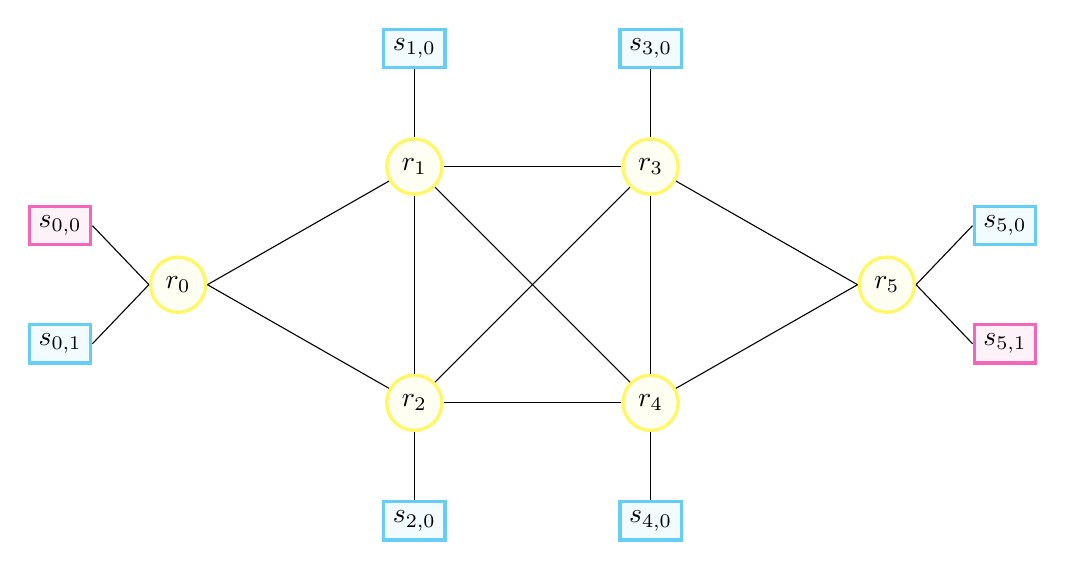
\begin{tikzpicture}[
        router/.style={circle, draw=yellow!60, fill=yellow!5, very thick, minimum size=3.5mm},
        nef_router/.style={circle, draw=red!60, fill=red!5, very thick, minimum size=3.5mm},
        switch/.style={rectangle, draw=cyan!60, fill=cyan!5, very thick, minimum size=2.5mm},
        monitor/.style={rectangle, draw=magenta!60, fill=magenta!5, very thick, minimum size=2.5mm},]
        
        % Routers
        \node[router] (r0) at (-4.5,0)    {$r_0$};
        \node[router] (r1) at (-1.5,1.5)  {$r_1$};
        \node[router] (r2) at (-1.5,-1.5) {$r_2$};
        \node[router] (r3) at (1.5,1.5)   {$r_3$};
        \node[router] (r4) at (1.5,-1.5)  {$r_4$};
        \node[router] (r5) at (4.5,0)     {$r_5$};
        
        %Switches
        \node[monitor](s00) at (-6,.75)   {$s_{0,0}$};
        \node[switch] (s01) at (-6,-.75)  {$s_{0,1}$};
        \node[switch] (s10) at (-1.5,3)   {$s_{1,0}$};
        \node[switch] (s20) at (-1.5,-3)  {$s_{2,0}$};
        \node[switch] (s30) at (1.5,3)   {$s_{3,0}$};
        \node[switch] (s40) at (1.5,-3)   {$s_{4,0}$};
        \node[switch] (s50) at (6,.75)   {$s_{5,0}$};
        \node[monitor](s51) at (6,-.75)   {$s_{5,1}$};
        %Links
        \draw[-] (r0.east) -- (r1);
        \draw[-] (r0.east) -- (r2);
        \draw[-] (r1) -- (r2);
        \draw[-] (r1) -- (r3);
        \draw[-] (r1.south east) -- (r4.north west);
        \draw[-] (r2) -- (r3);
        \draw[-] (r2) -- (r4);
        \draw[-] (r3) -- (r4);
        \draw[-] (r3) -- (r5.west);
        \draw[-] (r4) -- (r5.west);
        \draw[-] (s00.east) -- (r0.west);
        \draw[-] (s01.east) -- (r0.west);
        \draw[-] (s10) -- (r1);
        \draw[-] (s20) -- (r2);
        \draw[-] (s30) -- (r3);
        \draw[-] (s40) -- (r4);
        \draw[-] (s50.west) -- (r5.east);
        \draw[-] (s51.west) -- (r5.east);
    \end{tikzpicture}
    \caption{6 router network with 2 monitors located at $r_0$ and $r_5$ (Reprinted from page \pageref{fig:6routersample})}
    \label{fig:M6routersample}
\end{figure}\par
The total number of probe packets sent from monitors during analysis can be varied within our simulation tool. We refer to this number of probe packets sent as \textit{probing intensity}. At the end of the simulation the timestep each packet was sent from and received by a monitor is aggregated to give a distribution of packet transmission delays along that path.\par
To validate the accuracy of tomographic probing in nefarious settings, we consider the six-router network in \cref{fig:M6routersample}. The average of 50 simulations, each with a random set of nefarious routers, was taken over a range of probing intensities. The difference between inferred and true PDA was then averaged over all routers. Results are presented in \cref{fig:MPDAvarprobing}.\par
From this plot we can infer that the accuracy of network tomography increases proportionally to the number of probe packets sent. With 2,000 probe packets being sent a difference of $\approx 33\%$ between inferred and true values is seen. When the number of probe packets is increased to $\approx 12,000$ there is almost no difference between the true and inferred PDA values.\par
Therefore, network tomography enables accurate inference of router level PDA (and by extension buffer queue lengths). However, we anticipate the tolerance of discrepancies between the inferred and true values would impact the accuracy of nefarious router classification. We leave further study into trade offs between the cost incurred by sending additional probe packets, and the accuracy of nefarious router classification to future work.\par
Additionally, a two-sample Kolmogorov Smirnov test was conducted with a threshold of $\alpha=0.05$ and found no significant difference in accuracy of PDA inference between nefarious and non-nefarious routers. See \cref{ssec:MPDMseclection} for justification of our use of the packet delay average.
\begin{figure}[H]
    \centering
    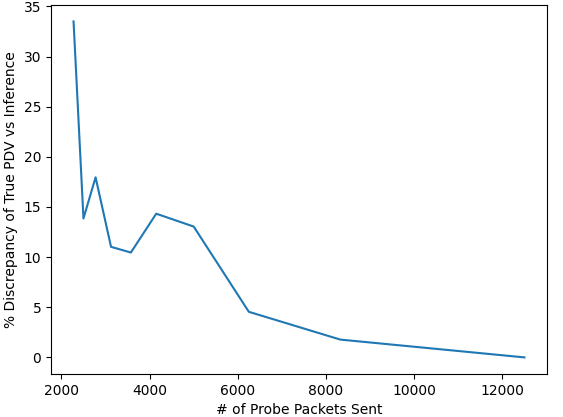
\includegraphics[width=0.8\textwidth]{figs/results/Probe_PDV_accuracy_plot.png}
    \caption{Accuracy of inference from true values over a range of probes sent.}
    \label{fig:MPDAvarprobing}
\end{figure}

\section{Packet Delay Metric Inference Validity}
\label{sec:MPDMinferencevalid}
To determine the validity of our core hypothesis (that packet delay metrics enable classification of routers probabilistically delaying packets), we again consider the six-router network from \cref{fig:M6routersample}. To observe the impact of nefarious behaviour on packet delay, six experiments were conducted with each router $r_0,\dots, r_5$ designed as nefarious in each experiment respectively.\par
Each experiment consisted of 50 trials over a range of holding probabilities for the nefarious router between 0 and 1. This was repeated for each router $r_0$-$r_4$ being designated as nefarious. In each trial, average packet delay statistics from 50 simulations were collected from each router every timestep, post queue stabilisation. Plots of router packet delay average (PDA) and variation (PDV) are shown in \cref{fig:Rvarnefrouter}.\par
Initially, all nefarious router packet delay metrics were grouped together in the analysis. However, as shown in \cref{tbl:MrouterPDAvars}, large variances in PDA, and consequently PDV, were observed in delay probabilities 0.2 - 0.5. Closer investigation revealed that this discrepancy of variances was between 3 groups of routers: $\{r_0,\ r_5\}$, $\{r_1,\ r_4\}$, and $\{r_2,\ r_3\}$. This grouping is validated by the variances shown in \cref{tab:Rallvars}.\par
From this we find that the intra-group variance is 100.60, 34.46, and 179.92 for each group respectively. However, they have an average inter-group variance of 862.99. Each group has a common feature: that its comprising routers are indistinguishable via their values in the adjacency matrix. Using these groupings it is clear that the nefarious router's PDA differs significantly from all other routers in the network. With a hold probability of 0.5 a nefarious router has PDA $\approx$3232 times larger than that of the 2nd largest PDA.\par
Of interest is the behaviour of $r_0$ and $r_5$ when nefarious, as although these routers connect to half as many routers as the others, their nefarious behaviour can still be inferred through PDA. This relationship enforces our conclusion that PDA metrics allow for nefarious router identification. We note that no routers in topologies from the SDNlib, nor Internet Topology Zoo, are indistinguishable via their values in the adjacency matrix. We therefore do not consider the impact of this nefarious router PDA grouping in our analysis.\par
As expected, when the nefarious router has a hold probability of 0, its PDV mimics that of a non-nefarious router. However, when a nefarious router has a very high hold probability $\gtrapprox 0.7$ we see again the PDV regresses to that of the rest of the network, this is corroborated by analysis in \cref{ssec:MPDMseclection}.\par
We anticipate that this behaviour is due to the use of variance as a metric. If a router is delaying all packets traversing it then its queue length will be consistently large or the queue will be completely full, varying little. If this hypothesis proves true, it follows that, although the PDV decreases significantly over a nefarious holding probability of 0.7, the PDA would continue to increase. PDA measurements from the same experimental trials in \ref{fig:MrouterPDA} show a clear monotonic increase between PDA and holding probability, conforming to our expectations.\par

\begin{figure}[H]
    \centering
    \begin{subfigure}{0.475\textwidth}
        \centering
        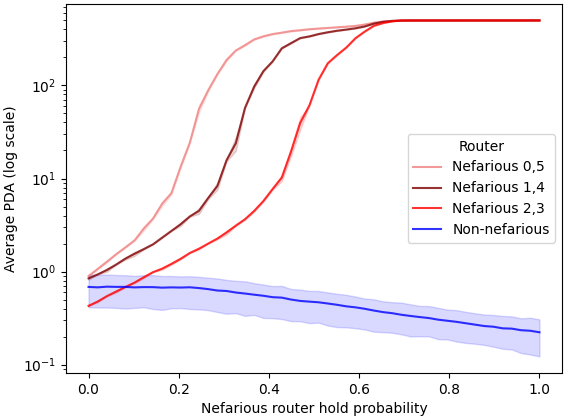
\includegraphics[width=\textwidth]{figs/results/grouped_summary_avg.png}
        \caption[]{Average Packet Delay}
        \label{fig:MrouterPDA}
    \end{subfigure}
    \begin{subfigure}{0.475\textwidth}
        \centering
        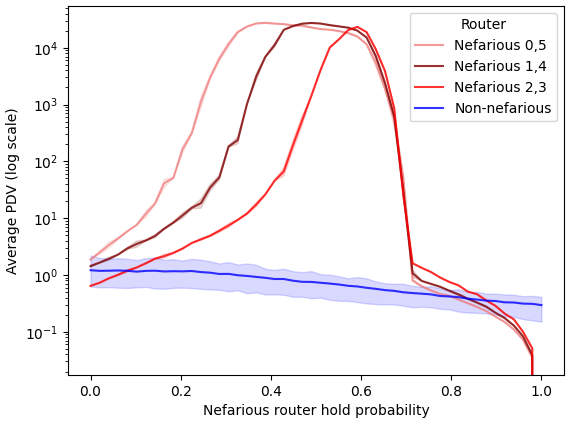
\includegraphics[width=\textwidth]{figs/results/grouped_summary_pdv.png}
        \caption[]{Packet Delay Variation}
        \label{fig:MrouterPDV}
    \end{subfigure}
    \caption{Average non-nefarious and grouped nefarious router packet metrics over a range of time-steps.}
    \label{fig:Rvarnefrouter}
\end{figure}
\sisetup{retain-zero-exponent}
\begin{table}[H]
 \centering
  \begin{tabular}{@{}cS[table-format=1.2e1]@{}}
   \toprule
    \textbf{Hold Probability} & \textbf{Nefarious router} \\
    \textbf{Range} & \textbf{PDA variance} \\
   \midrule
    {[}0.0, 0.1{)} & 3.03e-01  \\
    {[}0.1, 0.2{)} & 8.89e+00  \\
    {[}0.2, 0.3{)} & 1.49e+03  \\
    {[}0.3, 0.4{)} & 9.78e+06  \\
    {[}0.4, 0.5{)} & 8.54e+06  \\
    {[}0.5, 0.6{)} & 6.77e+05  \\
    {[}0.6, 0.7{)} & 1.03e+06  \\
    {[}0.7, 0.8{)} & 2.84e-01  \\
    {[}0.8, 0.9{)} & 3.13e-02  \\
    {[}0.9, 1,0{)} & 3.10e-03  \\
   \bottomrule
  \end{tabular}
  \caption{Variance of nefarious router PDA grouped by varying delay probabilities in the baseline six-router network.}
    \label{tbl:MrouterPDAvars}
\end{table}
\begin{table}[H]
    \centering
    \aboverulesep = 0pt
    \belowrulesep = 0pt
    \sisetup{table-number-alignment=center}
    \begin{tabular}{l|S[table-format=1.2e1]S[table-format=1.2e1]S[table-format=1.2e1]S[table-format=1.2e1]S[table-format=1.2e1]S[table-format=1.2e1]}
        \toprule
        {\backslashbox{$r_i$}{$r_j$}} & {$r_0$} & {$r_1$} & {$r_2$} & {$r_3$} & {$r_4$} & {$r_5$} \\
        \midrule
        {$r_0$} & 0.0e0  & 5.72e2 & 8.38e2 & 9.90e2 & 6.03e2 & 1.01e2 \\
        {$r_1$} & 5.72e2 & 0.0e0  & 5.58e2 & 7.35e2 & 3.45e1 & 6.37e2 \\
        {$r_2$} & 8.38e2 & 5.58e2 & 0.0e0  & 1.80e2 & 5.74e2 & 9.34e2 \\
        {$r_3$} & 9.90e2 & 7.35e2 & 1.80e2 & 0.0e0  & 7.50e2 & 1.06e3 \\
        {$r_4$} & 6.03e2 & 3.45e1 & 5.74e2 & 7.50e2 & 0.0e0  & 6.67e2 \\
        {$r_5$} & 1.00e2 & 6.37e2 & 9.34e2 & 1.06e3 & 6.67e2 & 0.0e0  \\
        \bottomrule
    \end{tabular}
    \caption{PDA variance between each nefarious router pair $r_i$ and $r_j$}
    \label{tab:Rallvars}
\end{table}


\section{Identifying Nefarious Behaviour}
\label{sec:MNefidentification}
In our problem setting, nefarious behaviour is characterized by a router probabilistically \textit{delaying} packets by not forwarding them during a timestep. As noted in previous chapters, we refer to a router's probability of delaying a packet during a timestep as its \textit{hold probability}.\par
To classify a router as behaving nefariously, we require a metric that is impacted by this nefarious behaviour and identifiable using network tomography. In that regard, packet delay (serving as a proxy for router buffer queue length) is an appropriate metric. We therefore hypothesise information gained from packet delay metrics can be used to classify a router as exhibiting nefarious behaviour.\par
This section is divided into three sub-sections, the first of which describes our selection of packet delay metric. The subsequent two sections describe our method for evaluating produced nefarious router classifiers.\par
In \cref{ssec:MTruevalues} we consider classification using the true buffer queue length measurements from routers at simulation time. We do this to test our underlying assumption that a router's buffer queue length is influenced by its hold probability.\par
In \cref{ssec:MInferredvalues} we instead use packet delay averages from network tomography to classify routers as nefarious. Finally, also in \cref{ssec:MInferredvalues}, we present our approach to comparing the classifications using both inferred and true data sets under each case of assumptions.
  
\subsection{Packet Delay Metric Selection}
\label{ssec:MPDMseclection}
Using path level packet delay distributions, we compute path PDA and PDV with NumPy's (\cite{harris_array_2020}) vector operations. These metrics are substituted to each router's identifiability equation to compute router level metrics.\par
To determine whether use of PDA or PDV enables the most accurate inference of true router level metrics, we consider the six-router network in \cref{fig:M6routersample}. We note that a combination of these metrics may enable more accurate inferences to be drawn regarding hold probability, but leave this to future work.\par
As a router's queue buffer contains a history of packets sent to it, the length of the queue buffer determines how much information about packets a router can hold. To account for this variable information in our analysis, we take an average of router level PDA and PDV against hold probability from 50 simulations over a range of queue buffer lengths. Results are shown in \cref{fig:RvariedqlenPDM}. Note that a router with a hold probability of 0.0 is analogous to a non-nefarious router.\par
From this we see that router level PDA and hold probability exhibit a monotonically increasing relationship. In comparison, PDV for router queue lengths less than 5,000 reaches a maximum  after which it regresses back to 0. The hold probability which results in this maximum PDV is related to the router buffer queue length, with larger queue lengths causing the maximum PDV to occur at a greater hold probability. Both PDA and PDV values before this maximum follow a similar trend. However, for large hold probabilities, PDA is far greater than PDV.\par
This reduction in PDV for large hold probabilities is likely due to the router's buffer queue reaching saturation. Once full, the queue length varies very little, as, even with stochastic routing, the router will receive very few of packets. These few packets will be from either a connected switch or from adjacent routers. However, these adjacent routers will only forward packets when they believe a path via the device with the saturated buffer queue has the shortest expected queuing delay.\par
  \begin{figure}
      \centering
      \begin{subfigure}{0.475\textwidth}
          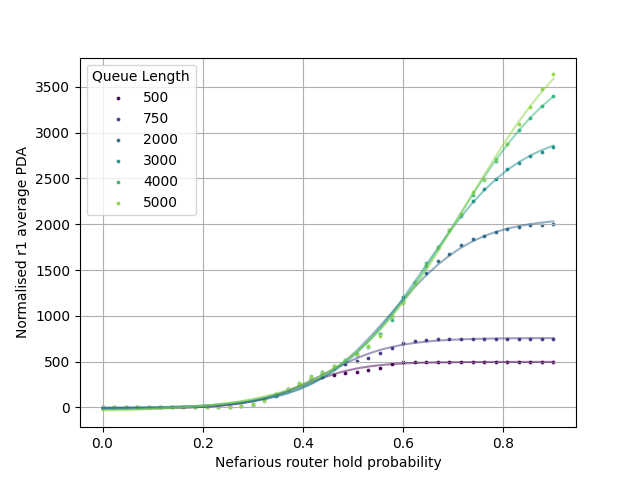
\includegraphics[width=\textwidth]{figs/results/qlen_fitting/qlen_PDA_lm.png}
          \caption{Packet Delay Average}
      \end{subfigure}
      \begin{subfigure}{0.475\textwidth}
          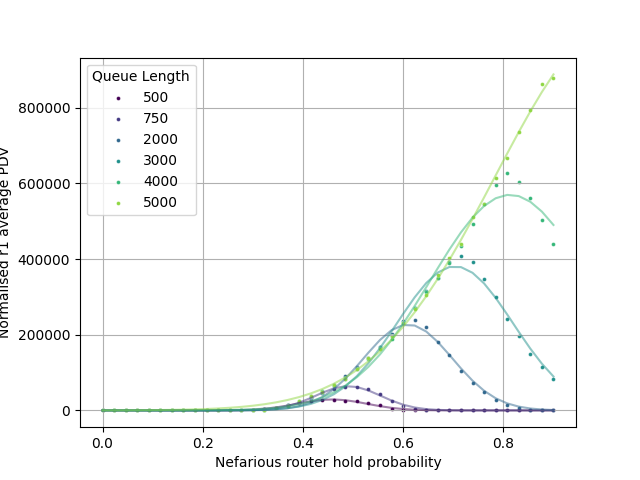
\includegraphics[width=\textwidth]{figs/results/qlen_fitting/qlen_PDV_lm.png}
          \caption{Packet Delay Variation}
      \end{subfigure}
      \caption{Plots of router level PDA and PDV over various hold probabilities.}
      \label{fig:RvariedqlenPDM}
  \end{figure}
As routers with very large hold probabilities have a higher chance of being nefarious, their identification by any produced classifier is imperative. Due to this we have opted to use PDA metrics for our classifier of nefarious nodes.\par
Additionally, from producing a function to fit the data points in this analysis, a parametric relationship was identified between router PDV and hold probability. From our use of various buffer queue lengths, a further relationship was observed between buffer queue length and the parameters of the optimally fitting function. This spurred an investigation into the possibility of using said relationship to directly compute router hold probability using PDA and network parameters (\textit{i.e. buffer queue length, traffic intensity, etc.}). We present this analysis in Appendix B and highlight this as an extremely promising avenue for further study.

\subsection{Nefarious Node Classification}
\label{ssec:MTruevalues}
In testing our sub-hypothesis of identifying nefarious routers, we construct three classifiers, each under a different set of assumptions. Each subsequent set of assumptions reduces the amount of information available for router classification. The sets of assumptions for each classifier are:
\begin{description}[labelindent=1cm]
  \item[Classifier 1:] Known router packet delay metrics with no nefarious routers (\textit{baseline metrics}) and complete distribution of router buffer queue length at each timestep.
  \item[Classifier 2:] Only known router packet delay metrics with no nefarious routers (\textit{baseline metrics}).
  \item[Classifier 3:] No additional assumptions.
\end{description}
The first set was chosen as it emulates a situation where network tomography yields perfectly accurate results. This serves as a test of whether, given full router level information, we are able to accurately classify nefarious routers.\par
The second and third sets emulate scenarios where results from network tomographic analysis presented in \cref{sec:Mnetworkprobing} are used for calculation. The second set additionally emulates a system under constant network monitoring. In this scenario, metrics with no nefarious routers can be viewed as system log files. The third set represents a scenario where these logs are not available, or where a new system is being analysed.\par
For classifiers one and two, we run additional simulations of each topology with no nefarious routers to serve as baseline metrics. We compute the mean of all metrics from these simulations, using these as the baseline metrics. With these baseline metrics and results from 500 blind trials with nefarious routers under each assumption set, we detail in turn how each classifier labels nefarious nodes, beginning with classifier one.\par
In assumption case one, we have two distributions of buffer queue lengths for each router, with only one known to have been collected from a non-nefarious router. To classify if a router is nefarious using these, we assume that a nefariously delaying router will have buffer queue lengths greater than an equivalent non-nefariously delaying router.\par
To compare these distributions we use SciPy's implementation of a one-tailed two-sample Kolmogorov-Smirnov test (\cite{chakravarti_handbook_1967}) in Python. To ensure the classification is accurate we select a p-value of 0.0 as required to label a router as nefarious. This means we tolerate virtually no chance of the result occurring by chance. We select this extremely low tolerance, as our assumptions in this test provide the most information possible.\par
In assumption case two, we do not have access to the complete queue buffer length distributions. Instead we utilise summary statistics obtainable from tomography; specifically PDA. Without the underlying distribution we are unable to use the Kolmogorov-Smirnov test as in classifier one.  However, it follows from our assumptions in case one that there will be a statistically significant difference in PDA between a nefarious and non-nefarious router.\par
To account for differences due to noise from stochastic routing, we use a standard deviation test for outliers. This test is shown in \cref{eq:stddev} where: $\mu$ and $\sigma$ are the mean and variance of the absolute differences between the baseline and potentially nefarious simulation for all routers; X is the given router's difference from baseline results; and $z$ is the threshold for being classified as nefarious. We vary the threshold for a router to be labelled as nefarious, and present the results in receiver operating characteristic (ROC) curves.\par
\begin{equation}
\label{eq:stddev}
  \frac{\mu-X}{\sigma}>z
\end{equation}
In the most restrictive scenario (case three), we have access to neither the underlying router buffer queue distribution nor a baseline of non-nefarious metrics. We therefore use PDA alone to label a router as nefarious, varying the PDA threshold required and again presenting results using ROC curves.\par
  
\subsection{Classification with Inferred Values}
\label{ssec:MInferredvalues}
We combine methods from \cref{sec:Mnetworkprobing} and \cref{sec:MNefidentification} to evaluate our overarching hypothesis that network tomography can be used to identify nefarious routers. This is analogous to cases two and three from \cref{ssec:MTruevalues}, where summary statistics of router queue lengths are used to classify routers as nefarious. Case one is not applicable, as the use of an underlying true distribution of router buffer queue lengths cannot be obtained with tomography. Instead, we present our method to test the efficacy of PDA (inferred through network tomography) as a metric for identifying nefarious routers. We firstly present our method under assumption case two, where system logs are available, and then case three, where they are not.\par
In assumption case two, where the baseline PDA of each router is known, we use the same methods as in \cref{ssec:MTruevalues} to assess if the router is nefarious. From network tomography we have the PDA at each router, analogous to the router's buffer queue length. We then compute the difference between the PDA of the baseline simulation and the simulation with unknown nefarious routers for each router in the network. We use a standard deviation test (\cref{eq:stddev}) to identify routers with a difference between the two simulations larger than a user-defined threshold. In assumption case three, with no baseline metrics to compare against, we use solely router-level PDA to classify nefarious routers.\par
For comparison of classifiers under each case of assumptions we consider both a graphic and a numeric presentation of their performance. For a qualitative evaluation we contrast the performance of each method using ROC curves produced by each classifier. For a quantitative comparison we consider three scenarios representing classifier use cases covering the spectrum of sensitivity and specificity requirements. These scenarios were selected because they allow us to evaluate the ROC curve at the upper right, middle, and lower left segments of the ROC curve respectively: 
\begin{description}[labelindent=1cm]
  \item[Scenario 1:] A false negative rate of < 10\% (sensitivity of 0.9)
  \item[Scenario 2:] A false negative rate < 30\%  and a false positive rate of < 50\% (sensitivity of 0.7 and specificity of 0.5)
  \item[Scenario 3:] A false positive rate of < 10\% (specificity of 0.9)
\end{description}
Scenario one represents a government network with a large budget and a low tolerance for unidentified compromised routers. Scenario two represents a budget restricted cloud provider with quality of service obligations around sensitivity and specificity of nefarious router detection. Scenario three represents an organisation monitoring a network of honeypot servers which wishes to avoid costly manual analysis of non-compromised machines.

\section{Optimising Inferential Accuracy}
\label{sec:Moptinferenceaccuracy}
In this section we discuss two candidate optimisations to network tomography and their implementation without our model. To understand these optimisations we represent network tomography as a four-stage pipeline (\cref{fig:tomographicpipeline}). In our approach to network tomography, we have used Ma's algorithm and Zheng's algorithm to compute an optimal set of monitors and probe paths. We therefore focus on evaluating the impact of optimisations to stages three and four of the pipeline.\par
In \cref{ssec:Mprobeallocation} we tackle the third stage of the pipeline. We conduct a test on a four-router network to make an informed design choice as to probe allocation. We then introduce an allocation of probe between paths, proportional to the number of routers each path is used to infer. The technical implementation of this \textit{proportional probe allocation} (PPA) is discussed with reference to our simulation's probabilistic injection of probes over paths.\par
In \cref{ssec:Mmetricnormilisation} we present a candidate optimisation to the fourth stage of the pipeline. Two unique factors which contribute to the size of a router's buffer queue, and therefore PDA, are postulated. These are the amount of traffic inbound to a router and the nefarious delaying behaviour of the router. As we aim to classify nefarious delaying behaviour, we attempt to account for the impact of inbound traffic by normalising each router's PDA by the router's degree.
\label{sec:Moptprobing}
\begin{figure}[H]
    \centering
    \tikzsetnextfilename{tomographicpipeline}
    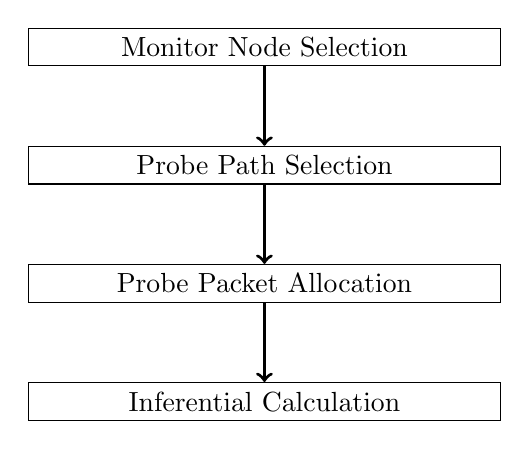
\begin{tikzpicture}
        \node[draw,minimum width=6cm] (A) at (0,4.5) {Monitor Node Selection};
        \node[draw,minimum width=6cm] (B) at (0,3) {Probe Path Selection};
        \node[draw,minimum width=6cm] (C) at (0,1.5) {Probe Packet Allocation};
        \node[draw,minimum width=6cm] (D) at (0,0) {Inferential Calculation};
        
        \draw[->, very thick] (A) -- (B);
        \draw[->, very thick] (B) -- (C);
        \draw[->, very thick] (C) -- (D);
    \end{tikzpicture}
    \caption{The Tomographic Pipeline.}
    \label{fig:tomographicpipeline}
\end{figure}

\subsection{Probe Allocation}
\label{ssec:Mprobeallocation}
Probes traversing different routers, and different probes traversing the same router, have an independent effect on the router's buffer queue length $q$. We can therefore develop an aggregation of all measurements in $\vec{q}$ assuming $r\in R, q_r \sim \mathcal{N}(0, \theta_r)$ where the variance $\theta_r$ is unknown.\par
Using this we aim to infer an estimation of $\vec{\theta}$ from our monitor-to-monitor measurements $\vec{q}$. To formalise our knowledge of the network from probing, we adapt a standard packet delay probability mass function from \cite{he_network_2021} where $\mathcal{M} = \sum_{r\in p}\theta_r$ in \cref{eq:pdvobservationmodel}. We denote the corresponding log-likelihood function as $\widehat{\mathcal{L}}(q, p)$.
\begin{equation}
\label{eq:pdvobservationmodel}
    f_{Q|\vec{\theta},\; \vec{\phi}}(q,\;p) = \phi_p \sqrt{2\pi\mathcal{M}}^{\ q^2/{2\mathcal{M}_r}}
\end{equation}
Using $\widehat{\mathcal{L}}(q, p)$ we are able to represent a network as a FIM. From this the CRB can be posed as a metric representing the lower bound on the accuracy of our inference. Using this CRB, we can evaluate the impact of different probe allocation schemes on the accuracy of network tomography.\par
Consider the example network in \cref{fig:fimex3routereg}. We define three probe paths $p_0$, $p_1$, and $p_3$ traversing $r_0\rightarrow r_2$, $\ r_1\rightarrow r_2$, $\ r_0\rightarrow r_2\rightarrow r_1$, and the reserve directions respectively.
\begin{figure}[H]
    \centering
    \tikzsetnextfilename{3routertopology}
    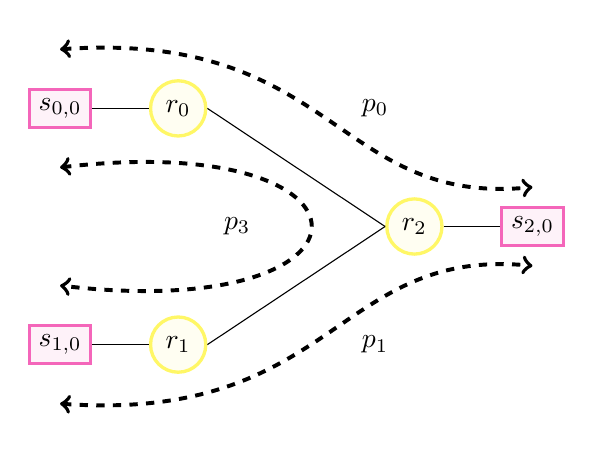
\begin{tikzpicture}[
        router/.style={circle, draw=yellow!60, fill=yellow!5, very thick, minimum size=3.5mm},
        nef_router/.style={circle, draw=red!60, fill=red!5, very thick, minimum size=3.5mm},
        switch/.style={rectangle, draw=cyan!60, fill=cyan!5, very thick, minimum size=2.5mm},
        monitor/.style={rectangle, draw=magenta!60, fill=magenta!5, very thick, minimum size=2.5mm},]
        
        % Routers
        \node[router] (r0) at (-1.5,1.5) {$r_0$};
        \node[router] (r1) at (-1.5,-1.5)  {$r_1$};
        \node[router] (r2) at (1.5,0) {$r_2$};
        %Switches
        \node[monitor](s00) at (-3,1.5)   {$s_{0,0}$};
        \node[monitor](s10) at (-3,-1.5)   {$s_{1,0}$};
        \node[monitor](s20) at (3,0)   {$s_{2,0}$};

        %Links
        \draw[-] (r0.east) -- (r2.west);
        \draw[-] (r1.east) -- (r2.west);
        \draw[-] (r0.west) -- (s00.east);
        \draw[-] (r1.west) -- (s10.east);
        \draw[-] (r2.east) -- (s20.west);
        
        % Probe path visualizations.
        \node at (1,1.5) {$p_0$};
        \draw[dashed, line width=.5mm, <->] (-3,2.25) .. controls (0.5,2.5) and (0.5,0.25) .. (3, 0.5);
        \node at (1,-1.5) {$p_1$};
        \draw[dashed, line width=.5mm, <->] (-3,-2.25) .. controls (0.5,-2.5) and (0.5,-0.25) .. (3, -0.5);
        \node at (-0.75,0) {$p_3$};
        \draw[dashed, line width=.5mm, <->] (-3,0.75) .. controls (1.25,1.25) and (1.25,-1.25) .. (-3, -0.75);

    \end{tikzpicture}
    \caption{Example 3 router network with probe paths explicitly noted.}
    \label{fig:fimex3routereg}
\end{figure}

We examine three different probe allocations between [$p_0,\:p_1$,\:$p_2$]. The first \textit{equivalent allocation} $\phi_0$ = [0.33, 0.33, 0.33] evenly distributes probes between all probe paths. The second \textit{proportional probe allocation} $\phi_1$ = [0.25, 0.5, 0.25] distributes probes to each path proportional to the number of routers that path is used to calculate. The third \textit{random allocation} $\phi_2$ = [0.8, 0.1, 0.1] was selected without use of a specific criteria so as to assess the impact of uninformed probe allocation.\par
As there are no nefarious routers, each router has an equal expected true PDA. Let these true PDAs be equivalent with $r_0=1, r_1=1, r_2=1$. The CRB of each probe allocation is then $\phi_0$=4.97, $\phi_1$=5.97, $\phi_2$=2.69. As $\phi_1$ results in the highest CRB it provides the highest minimum accuracy from probing. This also holds true when nefarious behaviour is considered.\par
Suppose the case of $r_1$ being nefarious with a $\frac{1}{3}$ probability of holding a packet any timestep. The CRB of each probing scheme is then $\phi_0$=1.51, $\phi_1$=4.24, $\phi_2$=2.05. Although each probing scheme performs worse than without the nefarious router, $\phi_1$ still exhibits the best performance.\par
We note for comparison that in the case of $r_1$ being nefarious an optimal probing allocation $\phi_{optimal}$ = [0.001, 0.499, 0.499] results in a CRB of 33.67. However, this optimal probing scheme only applies to this topology with a nefarious $r_1$. For other topologies the optimal probing scheme can only be found using an iterative traversal of the solution space. As we wish to apply the same probe allocation algorithm across multiple topologies, we will analyse the impact of PPA alone on our nefarious router classification.

\subsection{Metric Normalisation}
\label{ssec:Mmetricnormilisation}
The packet delay distribution of a router is a combination of the two contributors to its buffer queue length:
\begin{enumerate}
    \item The \# of packets received each timestep.
    \item The \# of packets sent each timestep.
\end{enumerate}
For non-nefarious routers, contributor \emph{2} is always a fixed rate of one packet per time step. If the router is nefarious, this rate is $<1$ proportional to the router's hold probability. As the rate of sending is not impacted by contributor \emph{1}, we hypothesise that accounting for variation of contributor \emph{1} between routers will enable more accurate inference of contributor \emph{2}, and subsequently of nefarious behaviour.\par
As \textit{traffic intensity} is constant across the network, we anticipate contributor \emph{1} to be proportional to the degree of each node. This is because the number of packets being received by a router each time step is the sum of packets received from each link. We therefore use \cref{eq:Mmetricnorm} to compute router level metrics for use in classification of nefarious routers.
\begin{equation}
    \label{eq:Mmetricnorm}
    \forall r\in R, \frac{PDA}{\sqrt{deg(r)}}
\end{equation}


\section{Summary}
In this chapter we have presented the methods we use to classify nefarious router behaviour, and have justified the design decisions behind these methods. In \cref{sec:Msimenvironment} we introduced three real-world ISP network data sets to be evaluated. Additionally, we discussed their programmatic representation, along with how they were parsed into this representation. We explicitly enumerated the functionality of produced tools for analysis and simulation of nefarious router classification using network tomography.\par
In \cref{sec:Mnetworkprobing} we presented our application of network tomography to our problem setting. Using a worked example, we analysed the accuracy of network tomography for inferred packet delay metrics. The accuracy of packet delay inference with network tomography was found to improve proportionally to the number of probe packets sent. A difference of 35\% was seen between true and inferred packet delays when 2,000 probe packets were sent between monitors. However, this difference was observed to approach 0\% as the number of probe packets was increase >12,000.\par
In \cref{sec:MPDMinferencevalid} we evaluated whether packet delays are a suitable indicator of routers probabilistically delaying packets. Results from simulation of a synthetic topology were provided. A statistically significant difference was observed between the packet delays of nefarious and non-nefarious routers.\par
In \cref{sec:MNefidentification} we discussed our use of network tomography to classify nefarious nodes in real-world ISP topologies. This section was broken into three sub-sections. In \cref{ssec:MPDMseclection} we addressed our design choice of packet delay metric used in classification. Specifically, we justified, using a worked example, our selection of PDA to classify nefarious routers over PDV (an alternate packet delay metric). In this example, PDV was found to be insufficient to identify routers with a high probability of delaying packets. As identification of these high-delay probabilities is desirable in classification of delaying routers, we chose to use PDA for this classification.\par
The second and third sub-sections explain the implementation of our classifiers, and the methods we use to evaluate findings. In \cref{ssec:MTruevalues} we focused on classification using true packet delay values. We introduced three different classifiers that we have developed, each under a different set of assumptions. In \cref{ssec:MInferredvalues} we focus on classification using packet delay values inferred using network tomography. We describe three scenarios with a range of sensitivity and specificity requirements, which we use to compare the performance of our classifiers.\par
Finally, in \cref{sec:Moptinferenceaccuracy}, we pose two candidate optimisations to network tomography. To select these optimisations, we represent the process of network tomography as a four-stage pipeline. We identify stages three and four (probe allocation over probe paths, and inferential calculation of metrics) as candidate areas for optimisation. We analyse the impact of different probe allocation schemes on the CRB of accuracy. We identified, \textit{proportional probe allocation} (PPA) as the most promising option for an optimal allocation scheme. This allocation scheme allocates probes to each path proportional to the number of routers each path is used to     calculate. Additionally, a normalisation of a router's PDA with respect to the router degree is presented as a potential method by which to better distinguish the impact of nefarious behaviour on PDA.\par